\chapter{\textbf{Applications of Belief Propagation Techniques}}
Belief Propagation Technique is used for performing inference on graphical models such as Bayesian Network and Markov Random Fields.\\Belief Propagation Technique calculates marginal distribution for each unobserved node, conditioning on any unobserved node.\\Some of the applications where Belief Propagation Techniques are used explained below.

\section{Efficient Belief Propagation for Early Vision}

Markov random field models provide a robust and unified framework for early vision problems such as stereo and image restoration. Inference algorithms based on graph cuts and belief propagation have been found to yield accurate results, but despite recent advances are often too slow for practical use.\\ In this paper some of the techniques  are used that substantially improve the running time of the loopy belief propagation .
\begin{enumerate}
  \item One of the techniques reduces the complexity of the inference algorithm to be linear rather than quadratic in the number of possible labels for each pixel, which is important for problems such as image restoration that have a large label set.
  \item second  technique speeds up and reduces the memory requirements of belief propagation on grid graphs.
  \item  A third technique is a multi-grid method that makes it possible to obtain good results with a small fixed number of message passing iterations, independent of the size of the input images.
\end{enumerate}


Taken together these techniques speed up the standard algorithm by several orders of magnitude. In practice results  obtained   are as accurate as those of other global methods (e.g., using the Middlebury stereo benchmark) while being nearly as fast as purely local methods.
\\The three techniques are used for speeding up the belief propagation by using Markov random fields for solving low level vision problems.
\\\\\ \\ The time necessary to compute a single message update from O (k 2 ) to O (k), where k is the number of possible labels for each pixel for the max-product formulation ie.linear rather than quadratic is possible.
\\By using max-product formulation and by grid graphs , The fast message updates to arbitrary discontinuity cost functions based on difference between labels and labels are embedded in some space but do not lie on a regularly spaced grid can be enhanced .



\section{Markov Network-based Unified Classifier for Face Identification }
In this research paper ,a novel unifying framework using a Markov network to learn the relationship between multiple classifiers in face recognition is explored. \\A  several complementary classifiers and assign observation nodes to the features of a query image and hidden nodes to the features of gallery images. each hidden node is connected to its corresponding observation node and to the hidden nodes of other neighboring classifiers.\\ For each observation-hidden node pair, to  collect a set of gallery candidates that are most similar to the observation instance, and the relationship between the hidden nodes is captured in terms of the similarity matrix between the collected gallery images. Posterior probabilities in the hidden nodes are computed by the belief-propagation algorithm.\\ The novelty of the proposed framework is the method that takes into account the classifier dependency using the results of each neighboring classifier. The  two different evaluation protocols, known and unknown image variation tests, using three different databases, which shows that the proposed framework always leads to good accuracy in face recognition.\\

When  a face image is used as as a query,  can retrieve several desired face images from a large image database,then  calculate many similarities of the query image and the
gallery images in the database, and the retrieved gallery images are ranked by similar orders. \\It is a one-to-many identification problem  and has many applications such
as searching similar face images in a database and face tagging in images and videos.\
\\Recent successful face recognition methods have attempted to merge several classifiers using multiple feature sets of different characteristics, as in component-based methods, which extract features from separate spatial regions , and heterogeneous feature-based methods which merge different domain features. \ These methods used the classifiers not only based on the different feature sets but also trained independently, and the similarity scores are merged with the predefined parameters. The parameter comes from the training database and it is not the best choice when the input image has different conditions. Note that these methods lead to good accuracy in face verification, but there is no specific framework for the one-to-many identification problem.
\begin{figure}
  % Requires \usepackage{graphicx}
  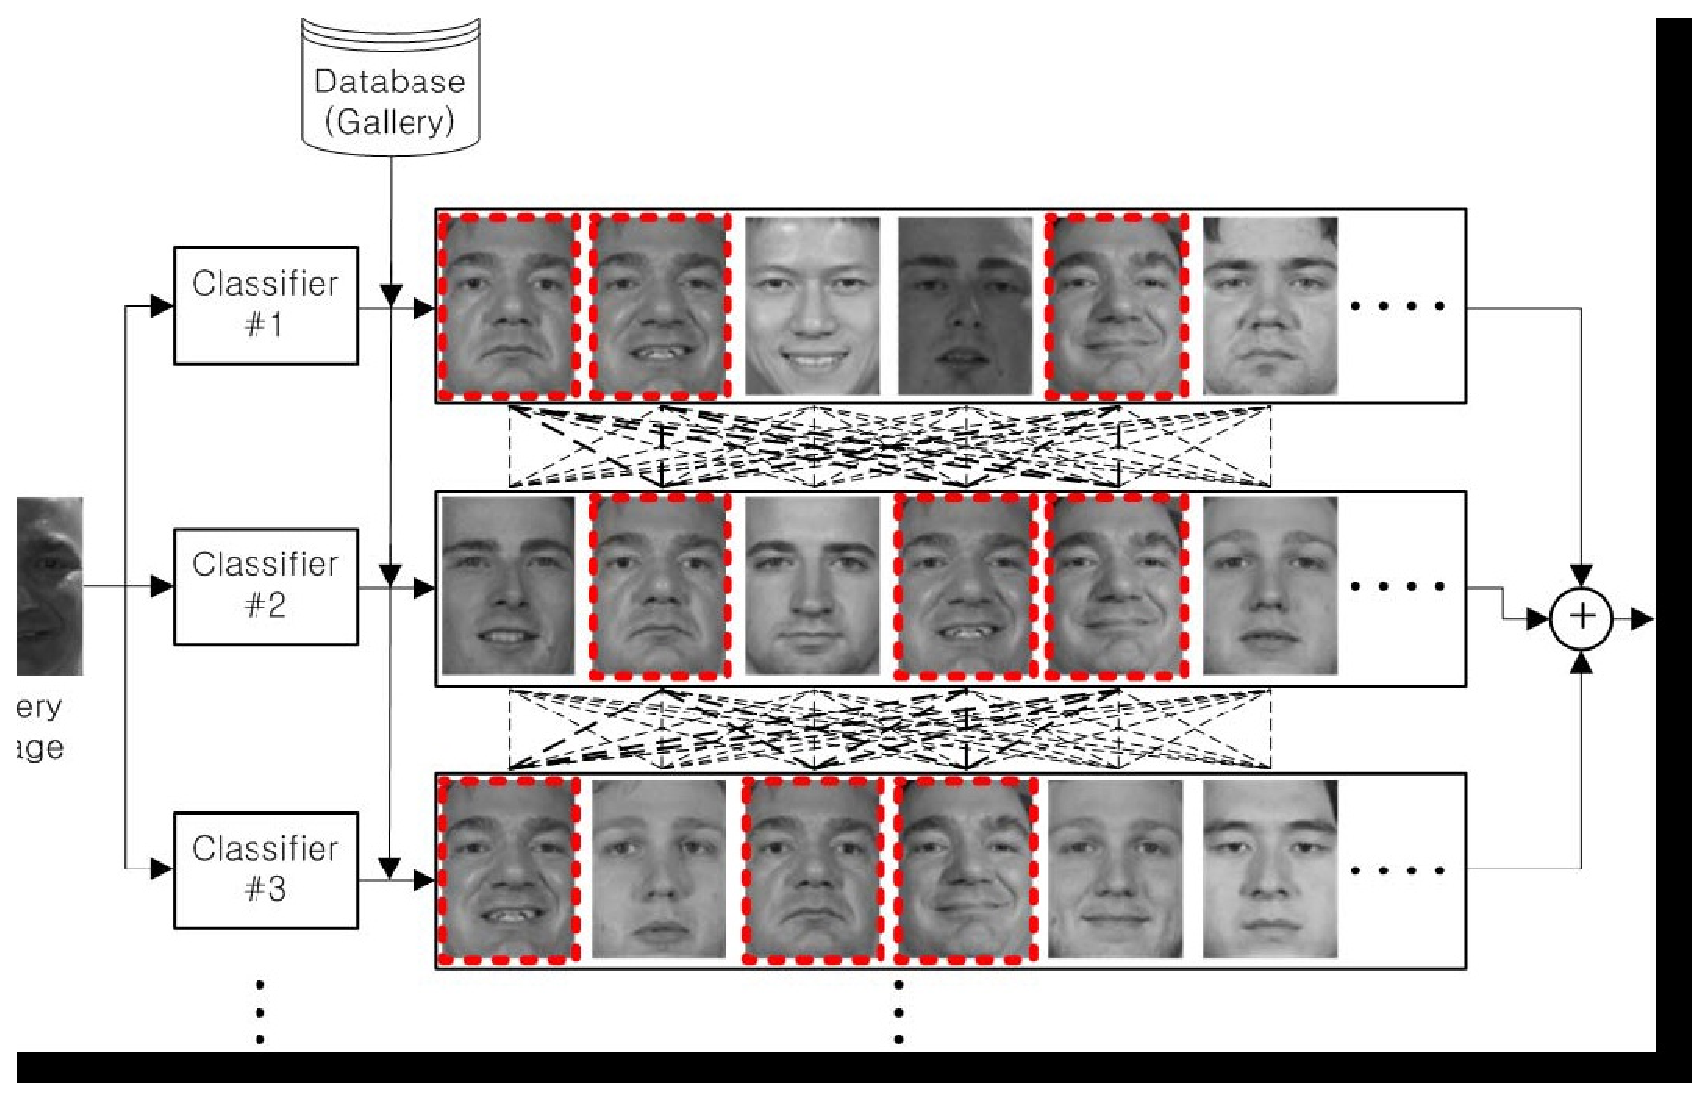
\includegraphics[width=4in]{face.eps}\\
  \caption{One-to-Many identification }\label{}
\end{figure}
\begin{figure}
  % Requires \usepackage{graphicx}
  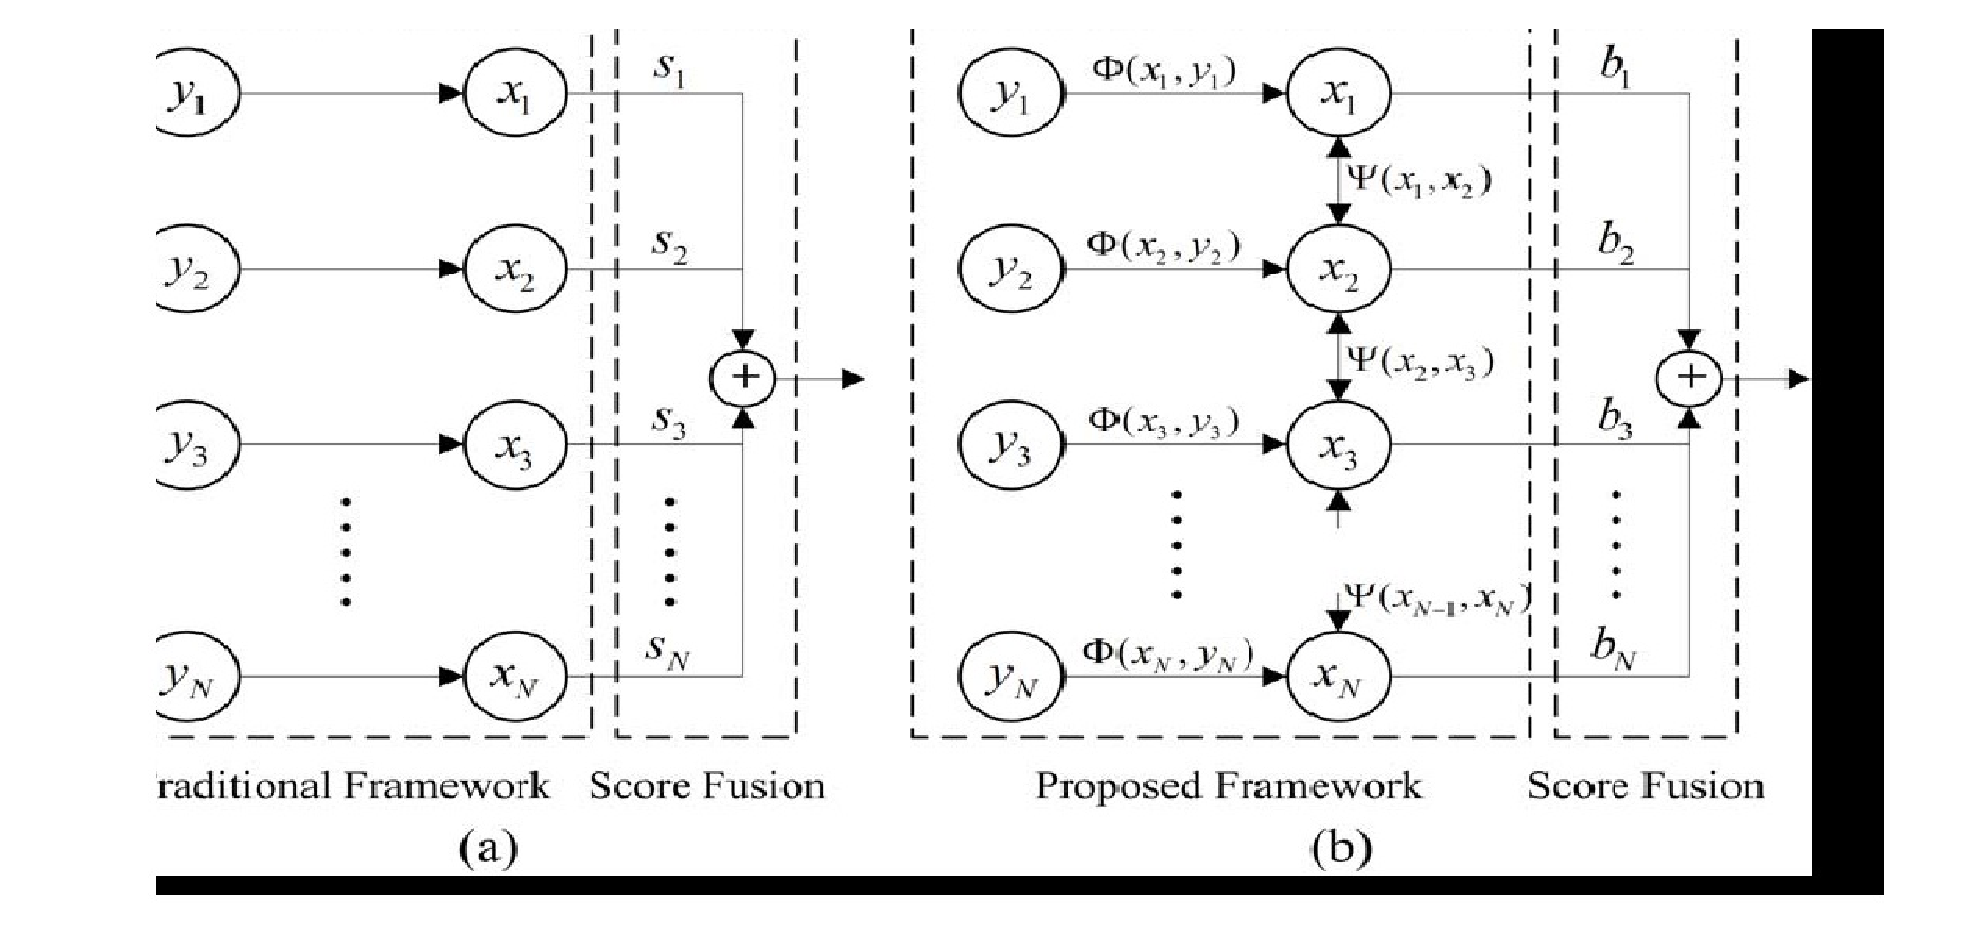
\includegraphics[width=4in]{classifier.eps}\\
  \caption{Traditional and proposed Frame Work}\label{}
\end{figure}

 \begin{itemize}
   \item In this paper, a novel recognition framework for the one-to-many identification issue is designed, and the simple concept is illustrated in Figure 3.1.
   \item First, assume that multiple classifiers have complementary characteristics, unify the multiple classifiers based not on the predefined weight values but on a Markov network, as summarized in Figure 3.2
 \end{itemize}

  For this purpose, assign one node of a Markov network to each classifier.The steps to find marginal probability by using Markov Fields for classifiers are as follows
  \begin{enumerate}
    \item Nodes are connected by lines, which represents the statistical dependencies
    \item For an observation node, we extract a feature from a query image using the corresponding classifier.
    \item At its paired hidden node,  the first retrieve n similar gallery samples from the database, and their orders are made by the similarity scores for the query face image.
  \item The multiple classifiers have their own lists of retrieved gallery images, which are not identical in general, thereby complementing the neighbor classifiers. Because the hidden nodes are connected by the network lines,
  \item The relationship of the connected nodes is learned by the similarity scores between the neighbor classifiers, and the scores are calculated by concatenating the two gallery features of the neighbor classifiers.
  \item The posterior probability at each hidden node is easily computed by the belief-propagation algorithm. Finally, marginal probability for a score value at each classifier is calculated
  \end{enumerate}
 And also analyze the generalizability of the method using different multiple classifiers such as the Random Sampled Gabor (RSG) method, which consists of the simple and weak classifiers, and the Extended Curvature Gabor (ECG) method which consists of more complex and stronger classifiers.
\\The results obtained are for face recognition particularly for the one-to-many identification task, based on multiple classifiers gallery connected by a Markov network.The Markov network probabilistically models the relationships between a query and images and between neighboring gallery images.
The observation-hidden node pair retrieve the  similar gallery images from the database image.
\\The similarities between the retrieved gallery images gives the statistical dependency between the hidden nodes. Hence results obtained can be viewed as clustering-based face recognition.



\section{Efficient Loopy Belief Propagation using the Four Color Theorem}
Recent work on early vision such as image segmentation, image  denoising, stereo matching, and optical flow uses Markov Random Fields.\\ Although this formulation yields an NP-hard energy minimization problem, good heuristics have been developed based on graph cuts and belief propagation.\\ Nevertheless both approaches still require tens of seconds to solve stereo problems on recent PCs. Such running times are impractical for optical flow and many image segmentation and
denoising problems and review on  recent techniques for speeding them up.

Moreover in this research paper it shows that  how to reduce the computational complexity of belief propagation by applying the Four Color Theorem (FCT) to limit the maximum number of labels in the underlying image segmentation to at most four. This provides substantial speed improvements for large inputs, and this for a variety of vision problems, while maintaining competitive result quality.
\\\\\\ In this research paper two methods are developed based on graph cuts  and belief propagation .

 \begin{itemize}
   \item In the case of Belief Propagation (BP), a key reason for its slow performance is that the algorithm complexity is proportional to both the number
of pixels in the image, and the number of labels in the underlying image segmentation
which is typically high. If  limit the number of labels, its speed performance should improve greatly.
   \item
By modifying the propagation algorithms like can using a low number of placeholder
labels, that can reuse for non-adjacent segments. These placeholder labels
can then be replaced by the full set of actual labels.
   \item Since image segments
form a planar graph, they therefore require at most four placeholder labels by
virtue of the Four Color Theorem (FCT)  to still have different colors for
all adjacent segments.
 \item A joint optimization process provides a fast segmentation
through the placeholder labels and a fine grained labeling through the
actual labels.
 \item  The computational time is basically dependent on the number
of placeholder rather than actual labels.
 \end{itemize}
 Statement of Four Color Theorem (FCT) is that\begin{itemize}
                                                \item for any 2D map there is a four-color covering such
that contiguous regions sharing a common boundary (with more than a single
point) do not have the same color
                                                \item The consequence of this theorem is that when
an image, seen as a planar graph, is segmented into contiguous regions, there
are only four colors to be assigned to each pixel/node for all segments to be
surrounded only by segments of different colors .
                                              \end{itemize}

 Four-Color Theorem (FCT)based on the max-product
belief propagation technique can be used in early computer vision for solving
MRF problems where an energy is to be minimized.
\\The  Methods used in this research yield results that are comparable with other methods, but improve either the
speed for large images and/or large label sets (the case of image segmentation,
stereo matching and optical ow), or both the performance and speed (the
case of image denoising)
\\The Four Color Theorem principle is difficult to apply in cases where
the label set is discrete in the case for stereo matching and optical flow, where the
disparity cost function takes discrete, unrelated values.This causes slower
convergence, but proposed methods can solve  the above mentioned problems.





\section{Image Completion Using Efficient Belief Propagation
Via Priority Scheduling and Dynamic Pruning}
The problem of image completion can be defined as for a given an image which is incomplete, i.e., it has
missing regions (as shown in  Fig.3.1), try to fill its missing parts in such a way that a visually plausible outcome is obtained at
the end. Although stating the image completion problem is very simple, the task of actually trying to successfully solve it, is far from being a trivial thing to achieve. Ideally, any algorithm that is designed to solve the image completion problem should have the following characteristics:
\begin{enumerate}
  \item it should be able to successfully complete complex natural
images
  \item it should also be able to handle incomplete images with
(possibly) large missing parts
  \item all these should take place in a fully automatic manner, i.e.,
without intervention from the user.
\end{enumerate}

Also, ideally any image completion algorithm to be able to handle the related problem of texture synthesis, as
well. For any  given a small texture as input,  then asked to generate an arbitrarily large output texture, which maintains the visual characteristics of the input as shown in Fig. 3.1. It is exactly due to all of the above requirements that image completion is, in general, a very challenging problem.
Nevertheless, it can be very useful in many areas, e.g., it can be important for computer graphics applications, image editing,
film postproduction, image restoration, etc. It has, thus, attracted a considerable amount of research over
the last years.  There have been three main approaches so far, for dealing with the image completion problem
as shown in Fig. 3.2
\begin{enumerate}
  \item Statistical-based methods
  \item PDE-based methods
  \item Exemplar-based methods
\end{enumerate}
\begin{figure}
  % Requires \usepackage{graphicx}
  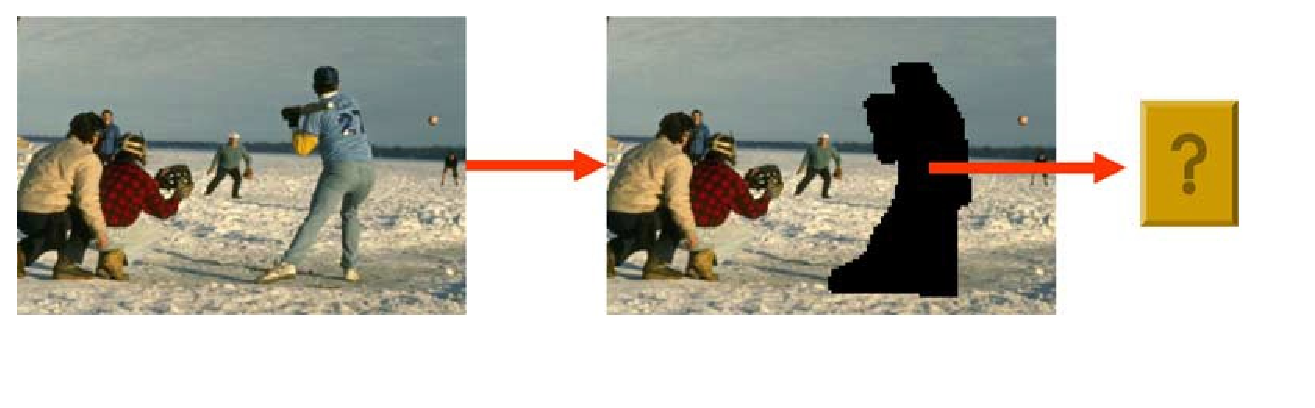
\includegraphics[width=6in]{prune1.eps}\\
  \caption{Object removal}\label{}
Object removal is just one of the many cases where image completion
needs to be applied. In the specific example shown, the user wants to remove a
person from the input image on the left. He, therefore, simply marks a region
around that person and that region must then be filled automatically so that a
visually plausible outcome is obtained.
\end{figure}
\begin{figure}
  % Requires \usepackage{graphicx}
  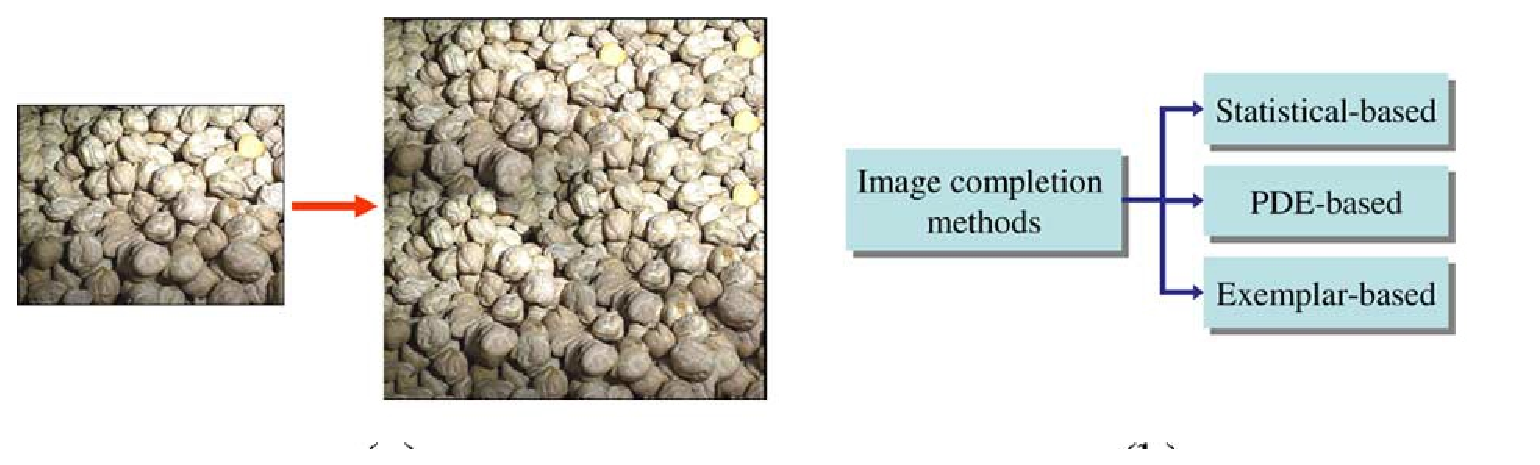
\includegraphics[width=6in]{prune2.eps}\\
  \caption{Texture synthesis problem and The three main approaches to image
Completion}\label{}
\end{figure}




\paragraph{Exemplar-Based Methods} : Exemplar-Based techniques, which actually have been the most successful techniques up to now. These methods try to fill the unknown region simply
by copying content from the observed part of the image. All exemplar-based techniques for texture synthesis
that have appeared until now, were either pixel-based or patch-based, meaning that the final texture
was synthesized one pixel, or one patch at a time (by simply copying pixels or patches from the observed image, respectively).
\\ A new exemplar-based framework  which treats image completion, texture synthesis, and image inpainting in a unified manner. All   image-editing tasks in the form of a discrete global optimization is used to avoid visually inconsistent results.
\\ The objective function of this problem is global optimization well-defined, and corresponds to the energy of a discrete Markov random field (MRF)
For efficiently optimizing this MRF, a novel optimization scheme, called priority belief propagation (BP) is used  which carries two very important extensions over the standard BP algorithm

  \begin{enumerate}
  \item \textbf{Priority-based message scheduling}
  \item \textbf{Dynamic label pruning}
\end{enumerate}

These two extensions work in cooperation to deal with the intolerable computational cost of BP, which is caused by the huge number of labels associated with  MRF. Moreover, both of  extensions are generic, since they do not rely on the use of domain-specific prior knowledge.They can, therefore, be applied to any MRF, i.e., to a very wide class of problems in image processing and computer vision.\\As one of  major limitation of the BP algorithm  is  its inefficiency in handling MRFs with very large discrete state spaces is considered to resolve by these extension techniques.

A novel optimization scheme which carries priority-based message scheduling and dynamic label pruning extensions for Belief Propagation known a priority BP is used.

The same optimization techniques can be used other types of completion problems such as video completion or geometric completion,constrained texture synthesis
\\ Priority-BP algorithm, which is a generic MRF optimization scheme can be used to other labeling problems  for which the large cardinality of their state-space causes them
to have a very high computational cost.


\section{Low Memory Cost Block-Based Belief Propagation For Stereo Correspondence}

Stereo correspondence is used in computer vision to find the depth among the cameras and objects.\\ This depth inference problem could be further transformed  to  a disparity inference problem by assuming that the cameras and objects are under epipolar geometry. The inferred disparity information could be widely applied to tracking, surveillance system, and multiview video coding \\\
The stereo matching algorithms can be roughly divided into two categories.
\\\
\begin{itemize}
  \item \textbf{local approaches}
  \item \textbf{global approaches}
\end{itemize}
\begin{itemize}
  \item Local approaches select disparities of image pixels using the information in a window. Therefore local approaches are faster than global approaches. However, it results in poor accuracy since the local approaches could not deal with textureless regions and occluded regions well due to the insufficient information in window.
  \item On the other hand, global approaches can handle the textureless and occluded regions well by formulating disparity inference as an energy minimization problem
\end{itemize}

 \begin{itemize}
   \item The energy function usually has a smoothness constraint which represents a certain physical relationship between neighboring pixel pair.
   \item This  smoothness  constraint often enforces penalty on the energy function, if the labels (disparities or segments) of neighboring pixels are inconsistent.
   \item Among the global methods, 2-D optimization algorithms such as graph cut and belief propagation (BP)  have been applied quite successfully to optimize energy function.
\end{itemize}



\begin{figure}
  % Requires \usepackage{graphicx}
  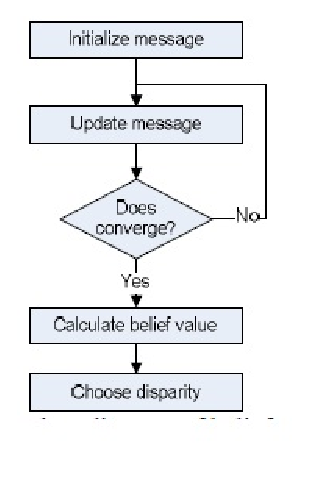
\includegraphics[width=2in]{block1.eps}\\
  \caption{Flow diagram of Belief Propagation}\label{}
\end{figure}
The flow chart  for Belief Propagation is shown in figure 3.5
 The BP algorithms construct 2-D graph structures with nodes representing all the pixels in the disparity images to find the disparity map with energy closer to the global minima.\ However, the vast number of nodes in the 2-D graph  result in  extremely high computation complexity, thereby rendering 2-D optimization is too difficult to be directly implemented for real-time application.\\
A block-based BP algorithm that directly partitions an image into separated independent blocks. Thus, can reduce the memory size significantly due to block based computation. In addition, the independent blocks also enable parallel computation by multiple computation units. Moreover earlier convergence for each block can also improve the long running time.


\begin{figure}
   Requires \usepackage{graphicx}
 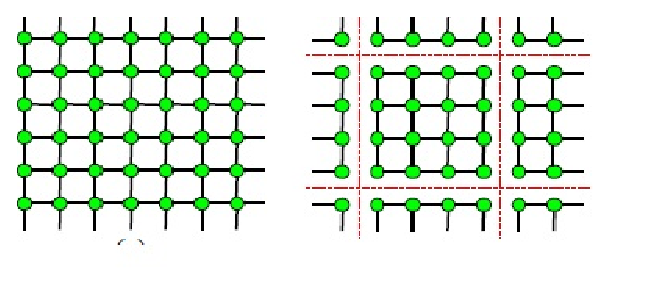
\includegraphics[width=4in]{block2.eps}\\
  \caption{graph of typical and block based BP}\label{}
2D Graph Model is shown in figure 3.6
\end{figure}

A new stereo matching algorithm partitions an image to block and optimizes with belief propagation technique.This method reduces memory storage size by 99
with good performance.
 To enhance the interaction  between neighboring blocks such that the independent block could extract useful information from  neighboring finished processing blocks are possible with block belief propagation.
\section{Task Parallel Implementation Of Belief Propagation In Factor Graphs}

Graphical models have been essential tools for probabilistic reasoning. Factor graphs  have emerged as a unified model of directed graphs (e.g. Bayesian networks) and undirected graphs (e.g. Markov networks).\\ A factor graph naturally represents a joint probability distribution that is written as a product of factors, each involving a subset of random variables.
Factor graphs have found applications in   Image processing,Bioinformatics and  Error-control decoding used in digital communications
Relation beteween  Factor graphs and Belief Propagation.
\begin{itemize}
  \item Inference is a problem of computing posterior probability distribution of certain variables given some value as observed or evidence variables.
  \item In factor graphs, inference proceeds with the well-known belief propagation algorithm . Belief propagation is a process of passing messages along the edges of a graph. Processing each message requires a set of operations with respect to the probability distribution of the random variables in a graph.
  \item Such distribution is represented by potential tables. The complexity of belief propagation increases dramatically as the number of states of variables and node degrees of a graph increase.
\end{itemize}

In many applications, such as digital communications, belief propagation must be performed in real time.\\ Therefore, parallel techniques are needed to accelerate the inference.Many parallel techniques have been proposed for belief propagation in factor graphs.\\ Parallelizing belief propagation in acyclic factor graphs still remains a challenging problem due to the precedence constraints among the nodes in the graphs. \\ Task scheduling is used in parallel computing is an efficient tool  for linear algebra problem on general-purpose multi-core processors.
The  methods used for  implementation of Belief Propagation using factor graphs are task dependency graph is used  by using a dynamic task scheduler.


\section{ Hardware-Efficient Belief Propagation}
Loopy belief  propagation (BP)  is  an  effective solution for  assigning labels to  the  nodes of  a  graphical model such as the Markov random field (MRF),
\begin{itemize}
  \item But it requires high memory, bandwidth, and computational costs.
\end{itemize}

The loopy BP has been widely applied to

\begin{itemize}
  \item Stereo matching
  \item Image denoising
  \item Image inpainting
\end{itemize}
  The success of BP is due to its regularity and simplicity. It uses a simple message  update  process  to iteratively refine the  beliefs  of labels for each node. A message sent from one node to another is updated according to neighboring messages and local energy functions, using simple arithmetic operations.\\
However, BP algorithms generally require a great amount of memory for storing the messages, typically on the order of tens to hundreds times larger than the input data.\ Besides, since each message is processed hundreds of times, the saving/loading of  messages consumes considerable bandwidth.\ Therefore, although BP may work on high-end platforms such as desktops, it cannot be applied to most consumer electronic devices that have limited memory, computational power, and energy. \ sequential procedure,  it  is  difficult to  utilize  hardware  parallelism  to accelerate BP.
The  two techniques  used
\begin{itemize}
  \item The first one is tile-based BP   splits the Markov random field (MRF) into many tiles and only stores the messages across the neighboring tiles. The memory and bandwidth required by this technique is only a fraction of the ordinary BP algorithms. But the quality of the results comparable to other efficient algorithms ,results are   tested by the publicly available Middlebury MRF benchmarks

  \item Second technique is that The fast message construction technique is based on the observation that many hypotheses used to construct the mesasages are repetitive. therefore, they only need to be computed once. This observation allows us to reduce the complexity of message construction from

\end{itemize}

Moreover, unlike previous sequential algorithms, the proposed algorithm can be easily parallelized.\
These techniques can be realized in both hardware and software. \ A software reference implementation compatible to  the  Middlebury  MRF  library  is  available  online,\ while two hardware the first one is a very large scale integration (VLSI) circuit and the second one a graphic processing unit (GPU) program are analyzed in this paper.



 The techniques used to develop a tile-based message passing and fast message construction  algorithm greatly reduced the memory, bandwidth, and computational costs of BP and enabled the parallel processing. With these two techniques  BP  can be  more suitable for low-cost and power limited consumer electronics.

\section{PMBP: PatchMatch Belief Propagation for Correspondence Field Estimation}
Patch Match is a simple, yet very powerful and successful method for optimizing Continuous labelling problems.
The algorithm has two main approaches  used are
\begin{itemize}
  \item The update of the solution space by sampling
  \item The use of the spatial neighborhood to propagate samples.
\end{itemize}
These approaches are related to steps in a specific form of belief Propagation in the continuous space, called Particle Belief Propagation (PBP). However, BP has thus far been too slow to allow complex state spaces.\\The two approaches used in this research yields a new algorithm called
Patch Match Belief Propagation for Correspondence Field estimation (PMBP), which is more accurate than Patch Match and orders of magnitude faster than PBP.
The methods used in research is novel realistic pair wise terms that provide Smoothness used for the recent Patch Match Stereo work.
The link between the popular PatchMatch method and the very well-known Belief propagation algorithm.

The link between the popular PatchMatch method and the very well-known Belief propagation algorithm  introducing additional pairwise terms, These approaches  can be  used as both in terms of applications, such as optical flow, as well as algorithms such as different forms of message passing e.g.  Treereweighted


\section{Learning continuous time Bayesian network classifiers}
Streaming data are relevant to use in finance,computer science,engineering while  they are becoming increasingly important to medicine and biology.


 The approach used for continuous time Bayesian network classifiers
  \begin{itemize}
    \item Continuous time Bayesian network classifiers are designed for analyzing multivariate streaming data when time duration of event matters.
    \item Structural and parametric learning for the class of continuous time  Bayesian network  classifiers are  considered  in  the  case where  complete  data is available.
    \item Conditional log-likelihood  scoring is developed for structural learning on continuous time Bayesian network classifiers.
   \item Results show that conditional  log-likelihood  scoring combined with Bayesian parameter estimation outperforms marginal log-likelihood scoring.
   \item Conditional log-likelihood  scoring becomes even more effective when  the amount of available data is limited.
\end{itemize}

Conditional log-likelihood scoring function is used  to learn continuous time Bayesian network classifiers from multivariate streaming  data.
Same function can be used for classifying multivariate trajectories in the case where the class is static .The quality of the classification performances also suggests to extend the Continuous Time Bayesian Network Classifiers to the clustering problem.
















